\section{System Design}


\subsection{Domain Model}

\subsubsection{Use Case Actors}
The main actor that can be considered in this system is the \textit{user}, since no administrative accounts are available, nor are they considered necessary at this moment.
\begin{itemize}
  \item User
  \begin{itemize}
    \item Responsibilities in the system
    \begin{itemize}
      \item -
    \end{itemize}
    \item Possibilities in the system
    \begin{itemize}
      \item Manage student groups 
      \item Create courses, quizes, questions.
      \item Generate random or predefined quizes
      \item Uploading of completed quizes
      \item Automatic marking of the scanned quizes
      \item Saving/printing of the generated quizes
    \end{itemize}
  \end{itemize}
\end{itemize}


\subsubsection{Use Case Diagram}
The use case diagram given below \ref{use_case_diagram}, shows the main actions that can be performed by an user inside the application. There are six direct actions presented for this purpose. The first one and the last two, counting from top to bottom, represent the managing part of the application, which includes the courses, quizes and questions. They have been chosen as actions to be described here, because togethe they comprise a big part of the application's functionality. This managing method is similar to a simplistic file manager system. You can do the basic operations in each compartment: create, delete, rename and view. The next action is about \textit{student group} and \textit{students} managing. It was not grouped together with the previous actions, because it does not have a direct contact with them in the front-end designed for the users. It practically does the same operations upon the created instances. The \textit{generate quiz} action is one of the two most essential actions, that the QTK is heavily relying on. From the user's point of view it represents a button that is present in all of the quizes' view pages. It is used to generate ready to print quizes, devised for specific purposes, that the user has in mind. This action also covers the action of choosing the options for generating those particular quizes. The \textit{upload quiz} action, is the second most important action, that simply represents the uploading of the completed quizes' scans to the application. This upload though, chains to itself two other indirect actions, that occur immediately after it is finished. These are the \textit{process quiz} action, which as the name suggests, process the image that was uploaded, and the \textit{mark quiz} action, which use the data aquired from the processing to give a rating to that quiz's filling.
\begin{figure}[!ht]
\centering
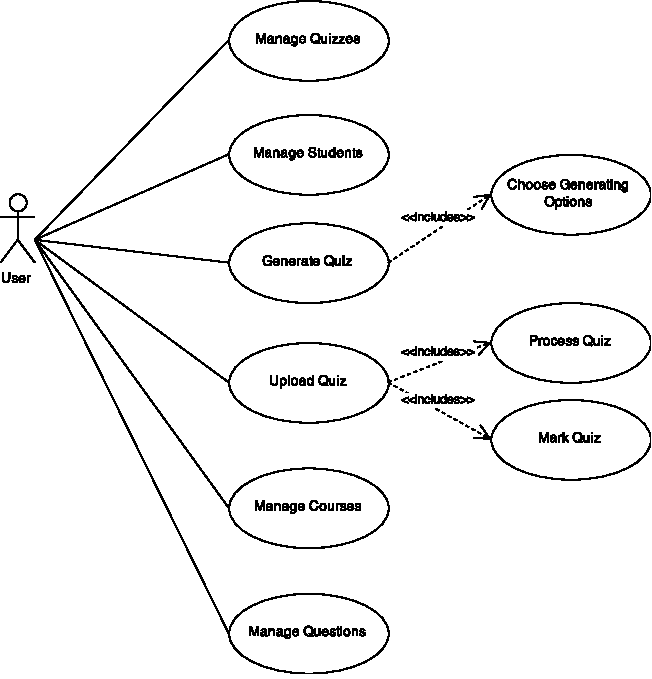
\includegraphics[scale=1.2]{use_case}
\caption{Use case diagram} \label{use_case_diagram}
\end{figure}

\subsubsection{Use Cases Description}
\begin{itemize}
  \item Register
  \begin{itemize}
    \item A teacher enters the system’s domain name in the browser
    \item A page appears, where the teacher clicks on the “Register” button
    \item The teacher is redirected to the register page
    \item He fills in the required fields and presses “Register”
    \item A message appears saying that an email has been sent to his address containing the confirmation link
    \item The teacher is redirected to the “Log in” page.
  \end{itemize}

  \item Log in 
  \begin{itemize}
    \item The user enters the system’s domain name in the browser. 
    \item A page appears, where the user must fill in his username and password and click the “Log in” button. 
    \item If authenticated successfully, the user will be redirected to his main page.
  \end{itemize}

  \item Create directories
  \begin{itemize}
    \item The user presses the “Create new” button, which is located above the directory list.
    \item A dialog window, that contains an input field  “Course name” and a button “Create”, appears.
    \item The user enters the name of  the directory and clicks “Create”
    \item This makes the dialog to vanish and the list to contain the new directory.
  \end{itemize}

  \item Delete directories
  \begin{itemize}
    \item The user marks the directories which are to be removed, by clicking on the box that is located to the left of the name of each directory. 
    \item Then he clicks on “Delete” button at the top of the list.
    \item A dialog appears, asking to confirm this action.
    \item The user clicks the “yes” button and the dialog disappears along with the chosen directories .
  \end{itemize}

  \item View a directory
  \begin{itemize}
    \item The user double-clicks the desired directory in the main page’s list
    \item The directory’s contents will appear instead of the courses list
  \end{itemize}  

  \item Create a quiz with manual input
  \begin{itemize}
    \item When user is in a course directory, he can create a new quiz
    \item He clicks the “Create new quiz” button
    \item A dialog  appears with two options: “Upload Quiz”, “Manual input”
    \item The user chooses the “Manual input”
  \end{itemize}

  \item Add question
  \begin{itemize}
    \item The user enters the question in the text area, presses the “Upload image” button to add an image to the question
    \item The user selects number of answers
    \item Fills in the answers
    \item Marks the correct answers
    \item Press “save” button
  \end{itemize}

  \item Create a tag
  \begin{itemize}
    \item When editing a question, the user presses “Add tag” button
    \item In the dialog, user writes in the text field the name of the tag
    \item User presses the “Create tag” button next to it
    \item The tag is created and it can be found in the dropdown list of the dialog
  \end{itemize}

  \item Add a tag to a question
  \begin{itemize}
    \item When editing a question, the user presses the “Add tag” button
    \item A dialog appears
    \item The user selects in the dropdown list the wanted tag
    \item The user clicks on the “Add tag” button
    \item The dialog disappears, and the tag is set
  \end{itemize}    

  \item Delete a quiz
  \begin{itemize}
    \item User selects from the list of quizes, the ones which should be deleted by checking the boxes.
    \item User clicks “delete” button
    \item User presses “yes” in the dialog window
    \item The selected quizes are deleted
  \end{itemize}    

  \item View a quiz
  \begin{itemize}
    \item User double-clicks a quiz from the course directory list
    \item The system shows all the questions of this quiz
  \end{itemize}    

  \item Edit a quiz
  \begin{itemize}
    \item When the user is in the quiz’s “view mode”, he can press the “edit” button near a question
    \item The question become editable
  \end{itemize}    

  \item Create a quiz with “upload” option
  \begin{itemize}
    \item The user clicks “create new quiz” button
    \item Presses “upload” button in the dialog window
    \item Then selects a file in the file manager window and presses “Upload”
    \item The quiz is created and the questions are created using the info in the file
  \end{itemize}

  \item Generate quiz
  \begin{itemize}
    \item In “view mode” of the quiz, the teacher presses “generate quiz” button
    \item A window with options appears
    \item The teacher selects the group for which the quiz is generated
    \item Checks the “random” option
    \item Presses “Generate”
    \item The new quiz file, containing all variants of the quiz is created in the course directory
  \end{itemize}

  \item Export quiz
  \begin{itemize}
    \item Teacher selects the generated file and presses the export button
    \item In the new dialog window, the teacher selects the destination directory
    \item Presses “Save”
    \item PDF file is saved on the machine
  \end{itemize}

  item Scan and process quizes
  \begin{itemize}
    \item The user clicks on “upload” button on the main page
    \item He selects the files and uploads them
    \item The system processes each file and get the necessary data from them
    \item The data is stored in the database
  \end{itemize}

  \item Create a student group
  \begin{itemize}
    \item The user clicks on the student group tab on the main page
    \item The system shows the list of groups and some buttons
    \item The user clicks on the create button
    \item The user is asked to enter the name of the group
    \item The user writes the name of the group and presses “Create”
    \item The new group appears in the list
  \end{itemize}

  \item Add a student to a student group
  \begin{itemize}
    \item The user double-clicks on a student group
    \item The system shows the list of students in that group
    \item The user presses on the “Add student” button
    \item He is prompted to enter the student’s name
    \item The user enters the name and clicks on “Add”
    \item The student appears in the list
  \end{itemize}
\end{itemize}

\subsection{Class Diagrams}
